\section{Introduction}

Dense visual prediction is a central problem in computer vision, because scene understanding often requires semantic labels, object identities, or structured regions at the pixel level. Representative milestones such as Fully Convolutional Networks (FCNs)~\citep{long2015fully}, Mask R-CNN~\citep{he2017mask}, and panoptic segmentation~\citep{kirillov2019panoptic} helped establish stable benchmarks and reliable task-specific pipelines under a closed-set paradigm, where the label space is fixed during training and unchanged at test time. Nevertheless, this paradigm leaves three limitations that are increasingly restrictive. It struggles with unseen categories and fine-grained concepts, it depends on costly dense mask annotation, and it cannot express user intents that are naturally described through free-form language.

Vision-language models (VLMs) offer a way to relax these restrictions by aligning visual regions with textual concepts. Contrastive Language-Image Pre-training (CLIP)~\citep{radford2021learning} showed that large-scale image-text supervision can support transferable visual recognition, which encouraged dense prediction systems to move from fixed labels toward text-defined category recognition. Early open-vocabulary segmentation methods, including Mask-adapted CLIP~\citep{liang2023ovseg}, Side Adapter Network (SAN)~\citep{xu2023san}, Open-Vocabulary Panoptic Segmentation with Text-to-Image Diffusion Models (ODISE)~\citep{xu2023odise}, and related recent studies~\citep{xshanOpenvocabularySemanticSegmentation2024,xwangUseUniversalSegment2024,shinhOpenvocabularySemanticSegmentation2024,yxchngAligningVisionLanguageModel2026}, transfer image-text semantics to pixels so that segmentation systems can recognize categories beyond the training label set. Yet semantic openness alone does not solve dense prediction. Open-vocabulary segmentation must preserve broad VLM semantics while recovering accurate boundaries, small structures, and region-level distinctions, which creates a persistent tension between semantic breadth and spatial precision.

\begin{figure}[t]
    \centering
    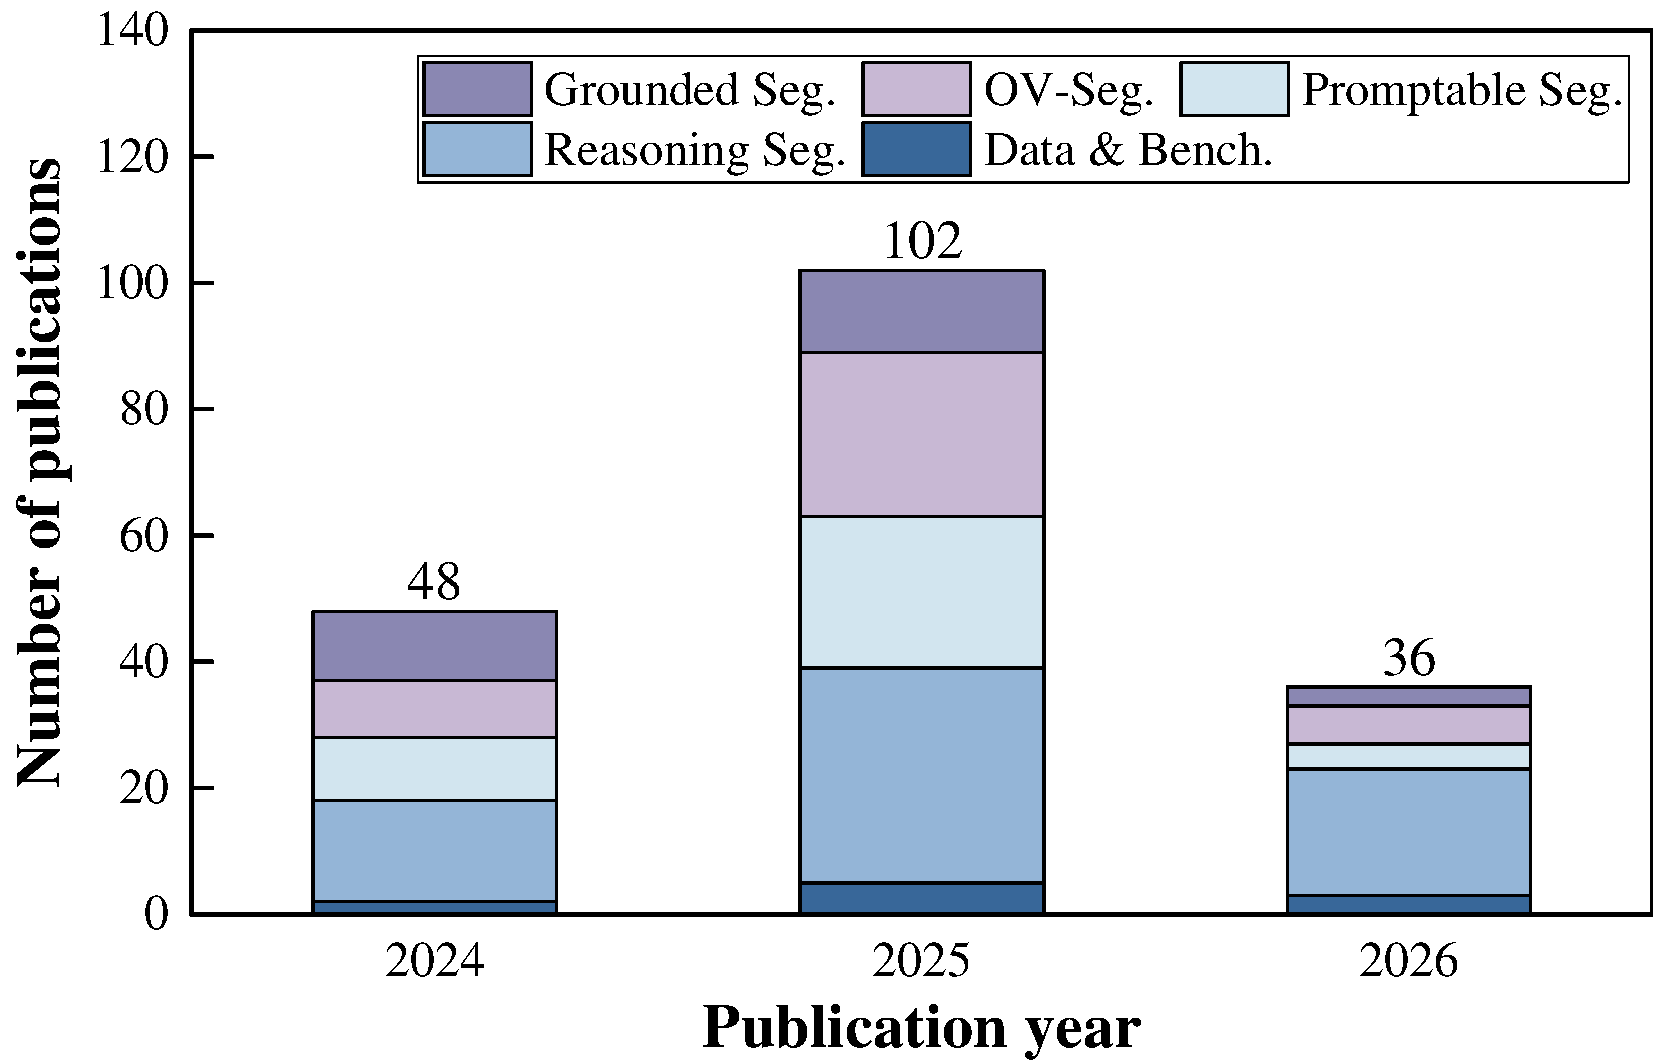
\includegraphics[width=0.85\linewidth]{Fig/Numberofpublications.pdf}
    \caption{Number of publications in the curated survey corpus from 2024 to 2026. The stacked bars group papers into grounded segmentation, reasoning segmentation, open-vocabulary segmentation, data and benchmarks, and promptable segmentation.}
    \label{fig-publication-statistics}
\end{figure}

\begin{figure*}[!t]
    \centering
    \includegraphics[width=0.98\textwidth]{Fig/intro_overview.png}
    \caption{Overview and taxonomy of the field evolution and technical routes reviewed in this survey. The top row summarizes the transition from closed-set segmentation to open-vocabulary, promptable, unified vision-language, and reasoning segmentation. The middle row groups the core technical routes. The bottom row places representative methods along the temporal development.}
    \label{fig-intro-overview}
\end{figure*}

Recent work has therefore developed several complementary routes. CLIP-based dense alignment adapts image-text representations to pixel prediction, proposal-then-classification pipelines classify candidate regions or masks, and the Segment Anything Model (SAM)~\citep{kirillov2023sam} together with Segment Anything Model 2 (SAM2)~\citep{ravi2024sam2} provides class-agnostic mask priors that separate mask generation from semantic assignment. SAM-based systems such as X-SAM~\citep{hwangXSAMSegmentAnything2026} and OpenWorldSAM~\citep{sgxiaoOpenworldsamExtendingSam22026} further extend promptable masks toward broader segmentation settings. In parallel, region-word and mask-text grounding methods connect linguistic units with spatial masks, supporting referring expression segmentation, grounded conversation, and fine-grained pixel-level visual understanding~\citep{xuPixelalignedLanguageModel2024,zhangLlavagroundingGroundedVisual2024,youFerretReferGround2024,rasheedGlammPixelGrounding2024}. These routes show that the field is no longer defined only by category recognition, but also by how language is grounded into spatial evidence.


The field has also shifted from naming visible categories to reasoning about what should be segmented. In reasoning segmentation, a query may refer to an implicit target through commonsense, spatial relations, multi-step instructions, false premises, or domain rules. Multimodal large language models (MLLMs) such as Large Language Instructed Segmentation Assistant (LISA)~\citep{lai2024lisa}, PixelLM~\citep{renPixellmPixelReasoning2024}, and Pixel Grounding Large Multimodal Model (GLaMM)~\citep{rasheed2024glamm} connect language generation with mask prediction through segmentation tokens, pixel decoders, or grounded multimodal conversation. Newer work further explores agentic reasoning, reinforcement learning (RL), preference optimization, and verifiable grounding to improve instruction following and mask faithfulness~\citep{luoConnectingDotsTrainingFree2026,zhuLensLearningSegment2026,zhouReasoningImplicitSelfsupervised2026,guoSeeingBelievingRichContext2026}. This shift expands segmentation into an interface where visual perception, language grounding, and structured reasoning must be modeled together.



The rapid concentration of recent work motivates a systematic review. As shown in Fig.~\ref{fig-publication-statistics}, the curated corpus contains 48 papers from 2024, 102 from 2025, and 36 from 2026, spanning open-vocabulary segmentation, promptable segmentation, grounded segmentation, reasoning segmentation, and dataset or benchmark construction. This distribution reflects a change in the center of gravity. Earlier studies emphasized text-defined labels and dense semantic alignment, whereas recent work increasingly targets promptable mask generation, instruction-guided segmentation, grounded multimodal dialogue, and reasoning-intensive pixel grounding. A survey is therefore needed to explain not only the growth of the literature, but also the technical routes that make these tasks comparable.

Fig.~\ref{fig-intro-overview} summarizes the taxonomy adopted in this survey. Across method families, the common system is composed of visual and textual representations that define the semantic space, mask generators or decoders that produce spatial regions, region or mask-text alignment mechanisms that bind language to pixels, and evaluation protocols that test openness, grounding, and reasoning. Based on these components, we organize the literature around technical routes rather than a paper-by-paper chronology. Open-vocabulary segmentation studies focus on dense semantic alignment, mask classification, and efficient adaptation. Promptable and grounded segmentation studies combine mask priors, region-word alignment, and language-guided prompting. Reasoning segmentation studies introduce MLLMs, explicit reasoning traces, grounded dialogue, and optimization with RL. Extended scenarios in video, 3D, remote sensing, medicine, affordance, and embodied grounding test whether these systems generalize beyond static 2D natural images~\citep{xuVideosegr1ReasoningVideo2026,chen3DDRESDetailed3D2026,libExploringEfficientOpenvocabulary2026,yanMedreasonerReinforcementLearning2026,wangAffordancer1ReinforcementLearning2026}.

Despite this progress, the literature remains difficult to compare. Different studies assume different prompt formats, label spaces, mask generators, training data, foundation backbones, and evaluation metrics. Some works evaluate open-vocabulary semantic segmentation with class-level labels, whereas others evaluate referring or reasoning segmentation with sentence-level instructions, mask-text pairs, or grounded conversations. Benchmark fragility further complicates comparison, because dataset names and label vocabularies may bias open-vocabulary evaluation, domain-specific imagery creates additional gaps, and MLLM outputs may be linguistically plausible but visually ungrounded~\citep{hhuangRenovatingNamesOpenvocabulary2024,libExploringEfficientOpenvocabulary2026,guoSeeingBelievingRichContext2026}. A useful survey must therefore clarify what methods exist, what each method assumes, what evidence supports its claimed capability, and where comparisons are not yet fair. We center this review on three recurring tensions, including semantic openness versus spatial precision, prompt and reasoning flexibility versus grounding faithfulness, and benchmark diversity versus fair comparison.

This survey provides a structured view of open-vocabulary and reasoning segmentation with vision-language foundation models. Its contributions are fourfold. First, we trace the development from closed-set dense prediction to open-vocabulary, promptable, grounded, and reasoning segmentation, clarifying the task assumptions behind each paradigm. Second, we summarize the common foundations, datasets, annotation granularity, and evaluation protocols that govern fair comparison. Third, we organize recent methods into technical families covering CLIP-based dense alignment, proposal and mask classification, SAM-based prompting with SAM2 extensions, region-word and mask-text grounding, MLLM-guided segmentation, and reasoning-to-mask generation. Fourth, we compare cross-family assumptions, benchmark settings, and trade-offs, then derive future directions on unified evaluation, faithful grounding, efficient adaptation, and generalization beyond static 2D natural images.

The rest of this survey is organized as follows. Section~2 introduces the background and task evolution. Section~3 presents the foundations of visual, textual, and mask representations. Section~4 reviews datasets, annotation types, and evaluation protocols. Sections~5 to~7 survey open-vocabulary segmentation, promptable and grounded segmentation, and reasoning segmentation. Section~8 discusses extended scenarios including video, 3D, remote sensing, medicine, affordance, and embodied grounding. Section~9 compares method families and benchmark limitations. Section~10 outlines future directions, and Section~11 concludes the survey.
